% LearningToOptimize ecosystem: which package depends on which.
%
% Every package depends on L2OCore (lib/L2OCore of this repository) and on
% nothing else of the ecosystem. Dashed boxes are planned packages; dashed
% arrows are planned dependencies or package extensions (weak dependencies).
% Content follows the "Packages" section of docs/src/design.md.
%
% Build: make -C docs/src/assets/diagrams/src
%   pdflatex -jobname=learningtooptimize--ecosystem ecosystem.tex          -> wide layout
%   pdflatex -jobname=learningtooptimize--ecosystem-compact ecosystem.tex  -> narrow layout
\documentclass[tikz,border=4pt]{standalone}
% Shared style of the LearningToOptimize diagrams: the palette, lane frames, cards,
% chips and glyphs of the paper-style TikZ figures (the same visual system as the
% PortfolioOpt.jl and DecisionRules.jl figures). Each figure \input's this file.
\usepackage{amsmath,amssymb,bm}
\usepackage[T1]{fontenc}
\usepackage[scaled=0.92]{helvet}
\renewcommand{\familydefault}{\sfdefault}
\usetikzlibrary{arrows.meta,shapes.geometric,shapes.symbols,calc,positioning,decorations.pathreplacing}

\definecolor{dTeal}{HTML}{1A9AA0}
\definecolor{dTealLine}{HTML}{3FB3B8}
\definecolor{dNavy}{HTML}{3F4C8C}
\definecolor{dInk}{HTML}{1E2235}
\definecolor{dRed}{HTML}{E4573D}
\definecolor{dCoral}{HTML}{E2765A}
\definecolor{dOrange}{HTML}{F4A93B}
\definecolor{dPeach}{HTML}{FBD9AC}
\definecolor{dPanel}{HTML}{EEF0F2}
\definecolor{dGray}{HTML}{8A90A0}
\definecolor{dNode}{HTML}{14A3A8}
\definecolor{dShadow}{HTML}{D5DAE3}

% \ifcompact is true when the job name ends in "-compact" (narrow layout).
\newif\ifcompact
\ifnum\pdfmatch{-compact$}{\jobname}=1 \compacttrue\fi

\tikzset{
  >={Stealth[length=5pt,width=4pt]},
  every node/.style={text=dInk},
  title/.style={anchor=west,font=\small,inner sep=0pt},
  head/.style={font=\small\bfseries,text=dNavy},
  note/.style={font=\itshape\footnotesize,text=dNavy},
  dnote/.style={font=\itshape\footnotesize,text=dCoral},
  code/.style={font=\ttfamily\footnotesize,text=dNavy},
  store/.style={cylinder,shape border rotate=90,aspect=0.28,fill=dPeach,draw=dOrange,
                line width=0.7pt,minimum width=0.95cm,minimum height=1.2cm,font=\normalsize},
  dia/.style={diamond,fill=dOrange,draw=none,minimum size=0.9cm,inner sep=0pt,aspect=1,
              font=\normalsize},
  lnode/.style={circle,fill=dRed,draw=none,minimum size=0.66cm,inner sep=1pt,
                text=white,font=\normalsize},
  card/.style={rectangle,rounded corners=4pt,fill=white,draw=dShadow,line width=0.6pt},
  sheet/.style={rectangle,rounded corners=3pt,fill=dPanel,draw=dShadow,line width=0.6pt},
  chip/.style={rectangle,rounded corners=3pt,fill=dPanel,draw=none,font=\small,
               inner xsep=4pt,inner ysep=3pt},
  ochip/.style={chip,fill=white,draw=dGray,dashed,line width=0.6pt},
  pchip/.style={chip,fill=white,draw=dGray!70,dashed,line width=0.5pt,text=dGray},
  fwd/.style={->,dTealLine,line width=0.8pt},
  tgt/.style={->,dOrange,line width=0.9pt},
  dual/.style={->,dCoral,dashed,line width=0.9pt},
  dep/.style={->,dTealLine,line width=0.8pt},
  pdep/.style={->,dGray,dashed,line width=0.7pt},
  nn/.style={circle,minimum size=0.26cm,inner sep=0pt,draw=dInk!70,line width=0.35pt},
}

% Lane frame in the paper style: two shadow copies behind a teal rounded frame.
\newcommand{\lane}[4]{% #1 x0, #2 y0, #3 x1, #4 y1
  \foreach \o/\c in {0.16/dShadow!60,0.08/dShadow}
    \draw[\c,fill=white,rounded corners=5pt,line width=0.6pt]
      (#1+\o,#2-\o) rectangle (#3+\o,#4-\o);
  \draw[dTealLine,fill=white,rounded corners=5pt,line width=0.9pt] (#1,#2) rectangle (#3,#4);}

% Plain card frame (no shadow copies), for problems and losses.
\newcommand{\cardbox}[4]{\draw[dShadow,fill=white,rounded corners=4pt,line width=0.6pt] (#1,#2) rectangle (#3,#4);}

% Network glyph on one sheet. #1 = centre, #2 = name prefix, #3 = number of stacked
% sheets behind (0, 1 or 2).
\newcommand{\net}[3]{%
  \begin{scope}[shift={(#1)}]
    \ifnum#3>1 \node[sheet,minimum width=1.9cm,minimum height=1.8cm] at (0.30,0.22) {};\fi
    \ifnum#3>0 \node[sheet,minimum width=1.9cm,minimum height=1.8cm] at (0.15,0.11) {};\fi
    \node[sheet,minimum width=1.9cm,minimum height=1.8cm,fill=white] (#2sheet) at (0,0) {};
    \foreach \y [count=\i] in {0.36,0,-0.36} \node[nn,fill=dGray!45] (#2in\i) at (-0.64,\y) {};
    \foreach \y [count=\i] in {0.58,0.29,0,-0.29,-0.58} \node[nn,fill=dNode] (#2ha\i) at (-0.21,\y) {};
    \foreach \y [count=\i] in {0.44,0.15,-0.15,-0.44} \node[nn,fill=dNode] (#2hb\i) at (0.21,\y) {};
    \node[nn,fill=dOrange] (#2out) at (0.64,0) {};
    \foreach \a in {1,...,3} \foreach \b in {1,...,5} \draw[dGray!60,line width=0.2pt] (#2in\a) -- (#2ha\b);
    \foreach \a in {1,...,5} \foreach \b in {1,...,4} \draw[dGray!60,line width=0.2pt] (#2ha\a) -- (#2hb\b);
    \foreach \a in {1,...,4} \draw[dGray!60,line width=0.2pt] (#2hb\a) -- (#2out);
  \end{scope}}

% Jacobian mask glyph: an n x d grid with a few entries selected. #1 = centre.
\newcommand{\maskgrid}[1]{%
  \begin{scope}[shift={(#1)}]
    \foreach \i in {0,...,4} \foreach \j in {0,...,3}
      \draw[dShadow,fill=white,line width=0.4pt] (\j*0.2-0.4,-\i*0.2+0.5) rectangle ++(0.2,-0.2);
    \foreach \i/\j in {0/1,1/3,2/0,3/2,4/1}
      \draw[dOrange,fill=dOrange,line width=0.4pt] (\j*0.2-0.4,-\i*0.2+0.5) rectangle ++(0.2,-0.2);
  \end{scope}}

% Code names inside italic notes stay upright.
\newcommand{\cmd}[1]{{\upshape\ttfamily #1}}

% Software-architecture helpers: package cards, type chips and chip rows.
\tikzset{
  pkg/.style={rectangle,rounded corners=4pt,fill=white,draw=dShadow,line width=0.6pt,
              align=center,inner xsep=5pt,inner ysep=4pt,font=\footnotesize},
  pkgcore/.style={pkg,draw=dTealLine,line width=0.9pt},
  pkgplan/.style={pkg,draw=dGray,dashed,text=dGray},
  tchip/.style={chip,font=\ttfamily\footnotesize,inner xsep=3pt,inner ysep=2.5pt},
  tplan/.style={tchip,fill=white,draw=dGray,dashed,line width=0.5pt,text=dGray},
  absname/.style={anchor=west,font=\ttfamily\footnotesize,text=dNavy,inner sep=1pt},
}
% \chiprow{x}{y}{style}{A,B,C}: chips left to right from (x,y), anchored west.
\newcommand{\chiprow}[4]{%
  \coordinate (cr@next) at (#1,#2);
  \foreach \t in {#4} {%
    \node[#3,anchor=west] (cr@last) at (cr@next) {\t};
    \coordinate (cr@next) at ($(cr@last.east)+(0.12,0)$);}}


\newcommand{\pk}[2]{{\small\bfseries #1}\\#2}

\begin{document}
\ifcompact
% ============================ narrow (phone) layout ============================
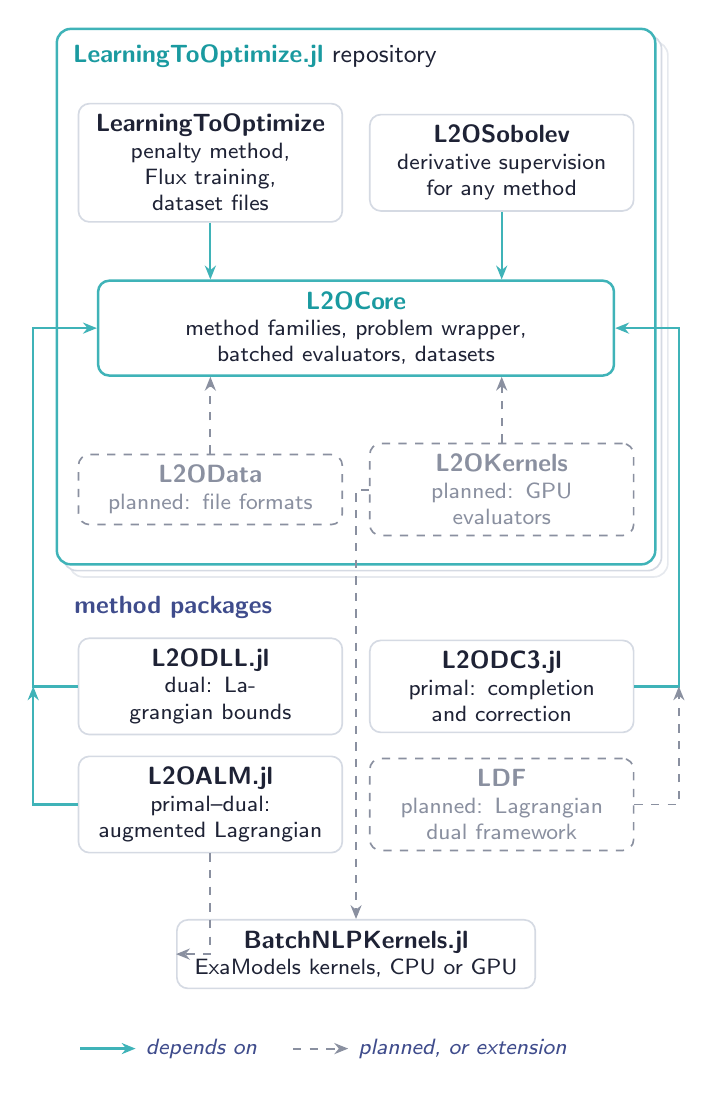
\begin{tikzpicture}
  \lane{0}{6.3}{7.6}{13.1}
  \node[title] at (0.2,12.75) {\textcolor{dTeal}{\bfseries LearningToOptimize.jl} repository};
  \node[pkg,text width=3.0cm] (lto) at (1.95,11.4) {\pk{LearningToOptimize}{penalty method,\\Flux training, dataset files}};
  \node[pkg,text width=3.0cm] (sob) at (5.65,11.4) {\pk{L2OSobolev}{derivative supervision\\for any method}};
  \node[pkgcore,text width=6.2cm] (core) at (3.8,9.3) {\pk{\textcolor{dTeal}{L2OCore}}{method families, problem wrapper,\\batched evaluators, datasets}};
  \node[pkgplan,text width=3.0cm] (dat) at (1.95,7.25) {\pk{L2OData}{planned: file formats}};
  \node[pkgplan,text width=3.0cm] (ker) at (5.65,7.25) {\pk{L2OKernels}{planned: GPU evaluators}};
  \draw[dep] (lto.south) -- (lto.south |- core.north);
  \draw[dep] (sob.south) -- (sob.south |- core.north);
  \draw[pdep] (dat.north) -- (dat.north |- core.south);
  \draw[pdep] (ker.north) -- (ker.north |- core.south);
  % method packages
  \node[head,anchor=west] at (0.1,5.75) {method packages};
  \node[pkg,text width=3.0cm] (dll) at (1.95,4.75) {\pk{L2ODLL.jl}{dual: Lagrangian bounds}};
  \node[pkg,text width=3.0cm] (dc3) at (5.65,4.75) {\pk{L2ODC3.jl}{primal: completion\\and correction}};
  \node[pkg,text width=3.0cm] (alm) at (1.95,3.25) {\pk{L2OALM.jl}{primal--dual:\\augmented Lagrangian}};
  \node[pkgplan,text width=3.0cm] (ldf) at (5.65,3.25) {\pk{LDF}{planned: Lagrangian\\dual framework}};
  \draw[dep] (dll.west) -- (-0.3,4.75) -- (-0.3,9.3) -- (core.west);
  \draw[dep] (alm.west) -- (-0.3,3.25) -- (-0.3,4.75);
  \draw[dep] (dc3.east) -- (7.9,4.75) -- (7.9,9.3) -- (core.east);
  \draw[pdep] (ldf.east) -- (7.9,3.25) -- (7.9,4.75);
  % kernels
  \node[pkg,text width=4.2cm] (bnk) at (3.8,1.35) {\pk{BatchNLPKernels.jl}{ExaModels kernels, CPU or GPU}};
  \draw[pdep] (ker.west) -- (3.8,7.25) -- (bnk.north);
  \draw[pdep] (alm.south) |- (bnk.west);
  \draw[dep] (0.3,0.15) -- (1.0,0.15) node[right,note] {depends on};
  \draw[pdep] (3.0,0.15) -- (3.7,0.15) node[right,note] {planned, or extension};
\end{tikzpicture}
\else
% =============================== wide layout ===================================
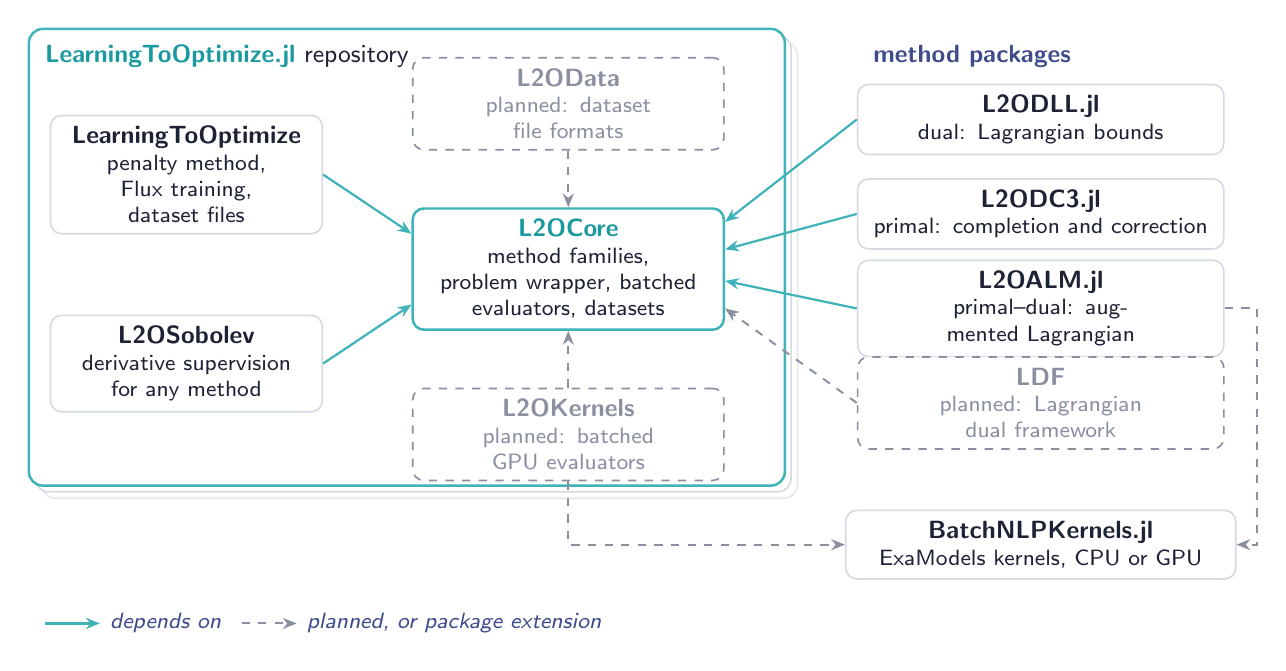
\begin{tikzpicture}
  \lane{0}{0}{9.6}{5.8}
  \node[title] at (0.2,5.45) {\textcolor{dTeal}{\bfseries LearningToOptimize.jl} repository};
  \node[pkg,text width=3.1cm] (lto) at (2.0,3.95) {\pk{LearningToOptimize}{penalty method,\\Flux training, dataset files}};
  \node[pkg,text width=3.1cm] (sob) at (2.0,1.55) {\pk{L2OSobolev}{derivative supervision\\for any method}};
  \node[pkgcore,text width=3.6cm] (core) at (6.85,2.75) {\pk{\textcolor{dTeal}{L2OCore}}{method families,\\problem wrapper, batched\\evaluators, datasets}};
  \node[pkgplan,text width=3.6cm] (dat) at (6.85,4.85) {\pk{L2OData}{planned: dataset file formats}};
  \node[pkgplan,text width=3.6cm] (ker) at (6.85,0.65) {\pk{L2OKernels}{planned: batched GPU evaluators}};
  \draw[dep] (lto.east) -- (core.west |- 0,3.2);
  \draw[dep] (sob.east) -- (core.west |- 0,2.3);
  \draw[pdep] (dat.south) -- (core.north);
  \draw[pdep] (ker.north) -- (core.south);

  % method packages
  \node[head,anchor=west] at (10.6,5.45) {method packages};
  \node[pkg,text width=4.3cm] (dll) at (12.85,4.65) {\pk{L2ODLL.jl}{dual: Lagrangian bounds}};
  \node[pkg,text width=4.3cm] (dc3) at (12.85,3.45) {\pk{L2ODC3.jl}{primal: completion and correction}};
  \node[pkg,text width=4.3cm] (alm) at (12.85,2.25) {\pk{L2OALM.jl}{primal--dual: augmented Lagrangian}};
  \node[pkgplan,text width=4.3cm] (ldf) at (12.85,1.05) {\pk{LDF}{planned: Lagrangian dual framework}};
  \draw[dep] (dll.west) -- (core.east |- 0,3.35);
  \draw[dep] (dc3.west) -- (core.east |- 0,3.0);
  \draw[dep] (alm.west) -- (core.east |- 0,2.6);
  \draw[pdep] (ldf.west) -- (core.east |- 0,2.25);

  % kernels
  \node[pkg,text width=4.6cm] (bnk) at (12.85,-0.75) {\pk{BatchNLPKernels.jl}{ExaModels kernels, CPU or GPU}};
  \draw[pdep] (ker.south) |- (bnk.west);
  \draw[pdep] (alm.east) -- (15.6,2.25) |- (bnk.east);

  \draw[dep] (0.2,-1.75) -- (0.9,-1.75) node[right,note] {depends on};
  \draw[pdep] (2.7,-1.75) -- (3.4,-1.75) node[right,note] {planned, or package extension};
\end{tikzpicture}
\fi
\end{document}
